\newcommand{\fw}{2.6cm}
\begin{figure*}
\centering
\begin{tabular}{ccccc|c|c}
%& & & & 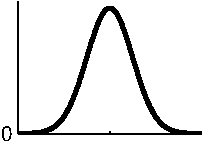
\includegraphics[width=\fw]{../figures/structure_examples/se_kernel} &  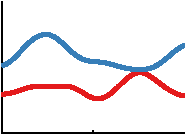
\includegraphics[width=\fw]{../figures/structure_examples/se_kernel_draws} & 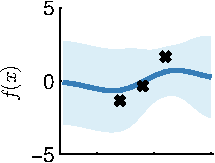
\includegraphics[width=\fw]{../figures/structure_examples/se_kernel_post} \\
%& & & & 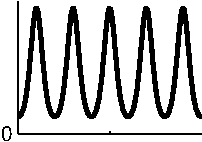
\includegraphics[width=\fw]{../figures/structure_examples/per_kernel} &  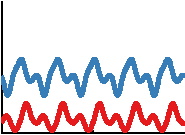
\includegraphics[width=\fw]{../figures/structure_examples/per_kernel_draws} & 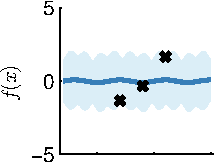
\includegraphics[width=\fw]{../figures/structure_examples/per_kernel_post} \\
%& & & & 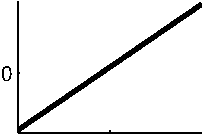
\includegraphics[width=\fw]{../figures/structure_examples/lin_kernel} &  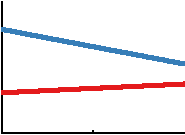
\includegraphics[width=\fw]{../figures/structure_examples/lin_kernel_draws} & 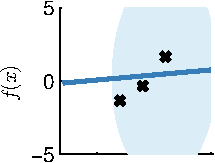
\includegraphics[width=\fw]{../figures/structure_examples/lin_kernel_post} \\
 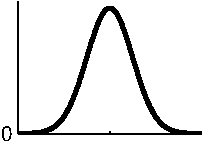
\includegraphics[width=\fw]{../figures/structure_examples/se_kernel} & $\times$ & 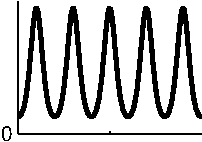
\includegraphics[width=\fw]{../figures/structure_examples/per_kernel} & = & 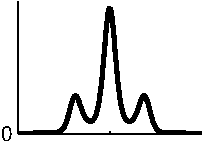
\includegraphics[width=\fw]{../figures/structure_examples/se_times_per} & 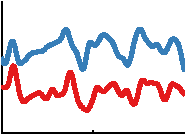
\includegraphics[width=\fw]{../figures/structure_examples/se_times_per_draws} & 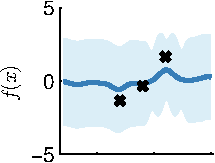
\includegraphics[width=\fw]{../figures/structure_examples/se_times_per_post} \\
  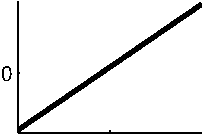
\includegraphics[width=\fw]{../figures/structure_examples/lin_kernel} & $\times$ & 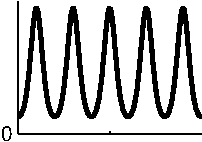
\includegraphics[width=\fw]{../figures/structure_examples/per_kernel} & = & 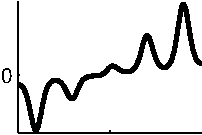
\includegraphics[width=\fw]{../figures/structure_examples/lin_times_per} & 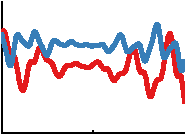
\includegraphics[width=\fw]{../figures/structure_examples/lin_times_per_draws} & 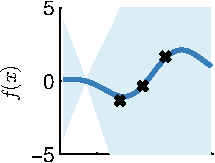
\includegraphics[width=\fw]{../figures/structure_examples/se_times_lin_post} \\
   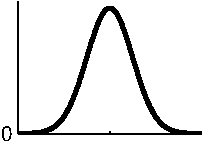
\includegraphics[width=\fw]{../figures/structure_examples/se_kernel} & $+$ & 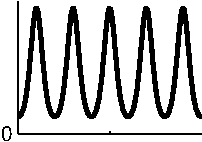
\includegraphics[width=\fw]{../figures/structure_examples/per_kernel} & = & 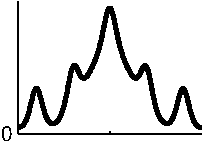
\includegraphics[width=\fw]{../figures/structure_examples/se_plus_per} & 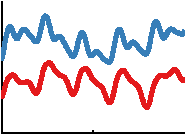
\includegraphics[width=\fw]{../figures/structure_examples/se_plus_per_draws} & 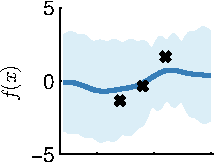
\includegraphics[width=\fw]{../figures/structure_examples/se_plus_per_post} \\
  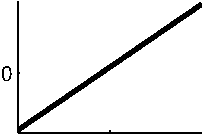
\includegraphics[width=\fw]{../figures/structure_examples/lin_kernel} & $+$ & 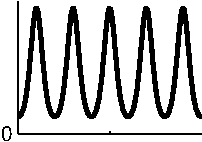
\includegraphics[width=\fw]{../figures/structure_examples/per_kernel} & = & 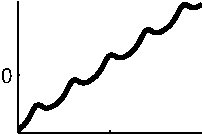
\includegraphics[width=\fw]{../figures/structure_examples/lin_plus_per} & 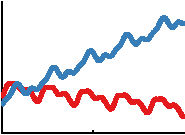
\includegraphics[width=\fw]{../figures/structure_examples/lin_plus_per_draws} & 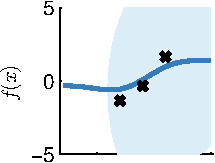
\includegraphics[width=\fw]{../figures/structure_examples/se_plus_lin_post} \\
   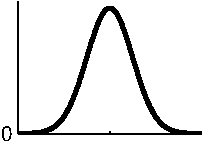
\includegraphics[width=\fw]{../figures/structure_examples/se_kernel} & $+$ & 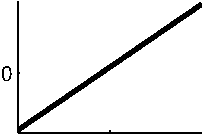
\includegraphics[width=\fw]{../figures/structure_examples/lin_kernel} & = & 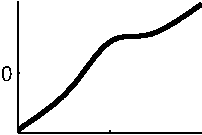
\includegraphics[width=\fw]{../figures/structure_examples/se_plus_lin} & 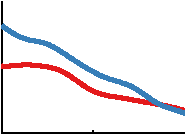
\includegraphics[width=\fw]{../figures/structure_examples/se_plus_lin_draws} & 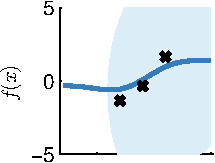
\includegraphics[width=\fw]{../figures/structure_examples/se_plus_lin_post} \\
   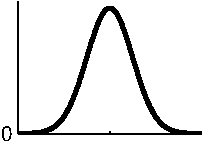
\includegraphics[width=\fw]{../figures/structure_examples/se_kernel} & $\times$ & 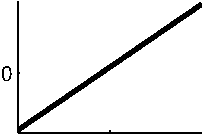
\includegraphics[width=\fw]{../figures/structure_examples/lin_kernel} & = & 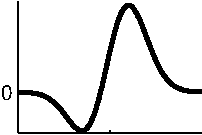
\includegraphics[width=\fw]{../figures/structure_examples/se_times_lin} & 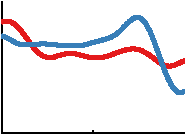
\includegraphics[width=\fw]{../figures/structure_examples/se_times_lin_draws} & 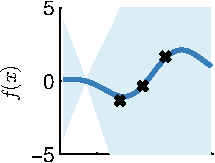
\includegraphics[width=\fw]{../figures/structure_examples/se_times_lin_post} \\
base kernel & & base kernel & & combined kernel & draws from GP & GP posterior
\end{tabular}
\caption{ A draw from a sum of kernels corresponds to a sum of draws from the base kernels.  A draw from a product kernel prior has weaker long-range dependencies, and less long-range structure.
}
\label{fig:kernels}
\end{figure*}